\section{MAC network and our proposed simplification}

\begin{wrapfigure}{r}[5pt]{0.4\textwidth}
	\vspace{-15pt}
	\centering
	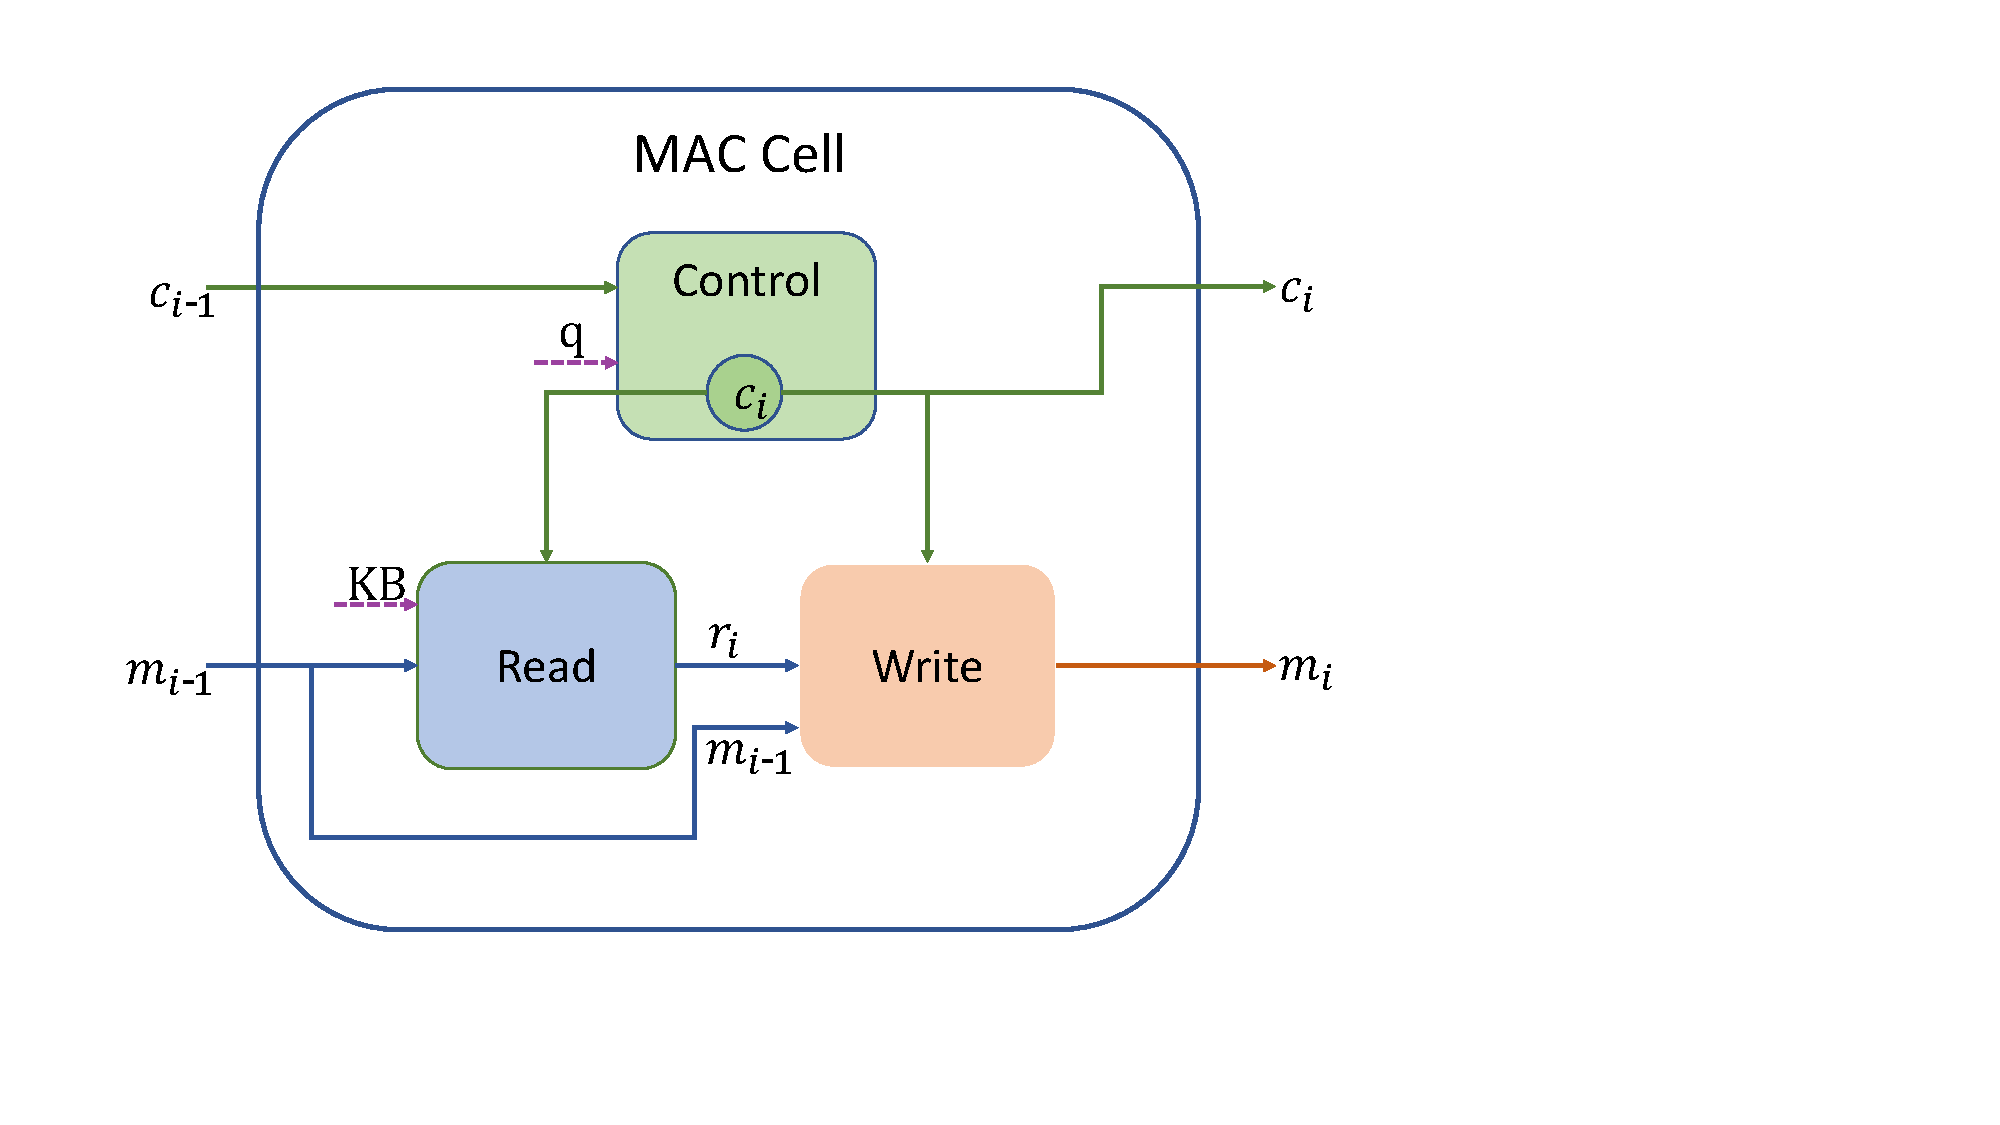
\includegraphics[width=\textwidth]{img/mac_cell.pdf}
	\caption{The MAC cell, reproduced on the basis of~\cite{hudson2018compositional}.}
	\label{fig:mac_cell}
	\vspace{-5pt}
\end{wrapfigure}

The MAC network~\cite{hudson2018compositional} is a recurrent model that performs sequential reasoning, where each step involves analyzing a part of the question followed by shifting the attention over the image.
The core of the model is the MAC cell, supported with an input unit that processes the question and image pair, and output unit which produces the answer.
The input unit  uses an LSTM~\cite{hochreiter1997long} to process the question in a word-by-word manner producing a sequence of \emph{contextual words} and a final \emph{question representation}.
Besides, the input unit utilizes a pre-trained ResNet~\cite{he2016resnet} followed by two CNN layers to extract a feature map (referred to as \emph{knowledge base}) from the image.

	
The MAC cell consists of a control unit, a read unit and a write unit (\Fig{fig:mac_cell}).
The control unit is updating the control state $c_i$ and drives the attention over the list of \emph{contextual words} $\cw$ taking into account the \emph{question representation} $q$.
Guided by $c_i$,  the read unit extracts information from the \emph{knowledge base} $\kb$ and combines it with the previous memory state $m_{i-1}$  to produce the \emph{read vector} $r_i$.
Finally, the write unit integrates $r_i$ and $m_{i-1}$ to update the memory state. Detailed equations are described in the next section.

%\begin{figure}[htbp]
%	\centering
%	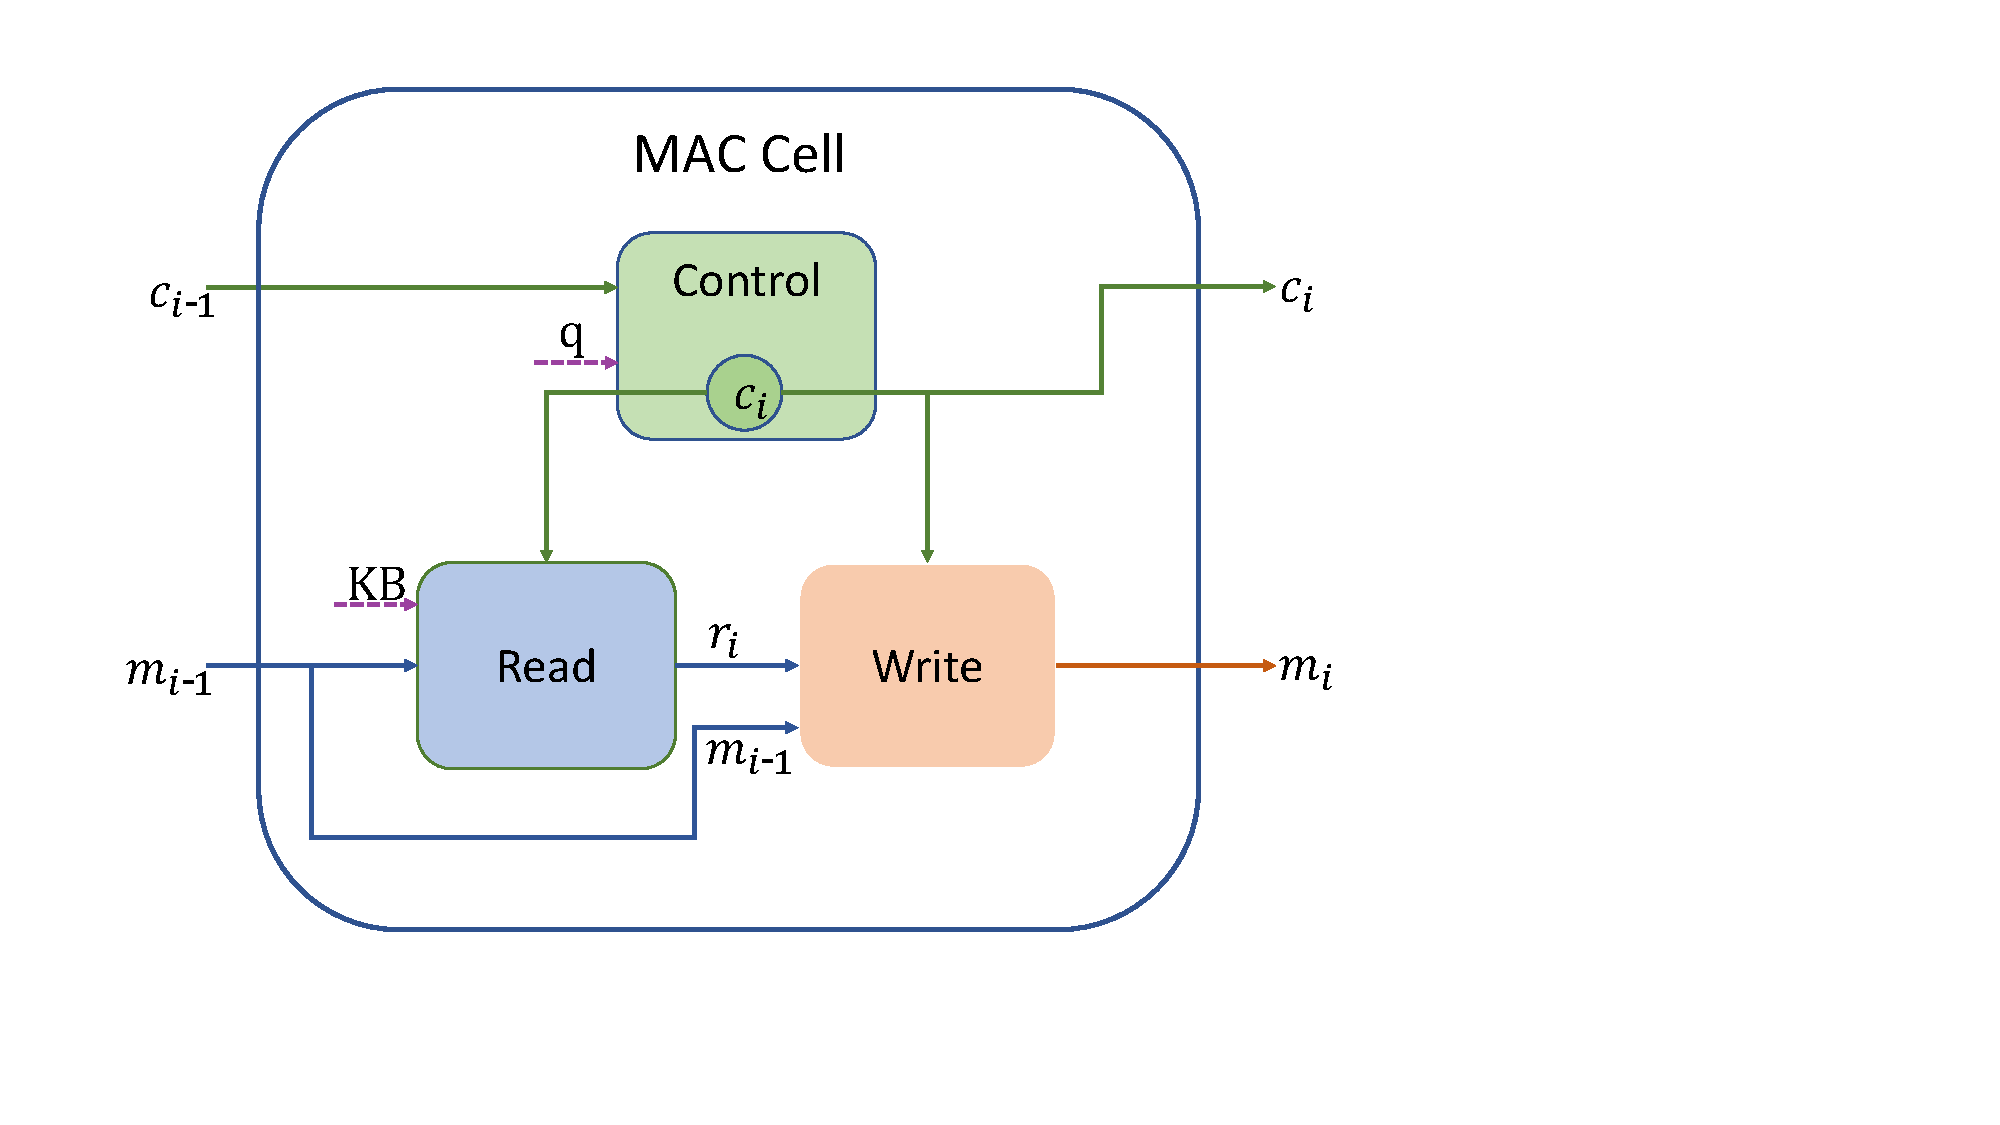
\includegraphics[width=0.4\textwidth]{img/mac_cell.pdf}
%	\caption{The MAC cell~\cite{hudsonManning18}}
%	\label{fig:mac_cell}
%\end{figure}
